\chapter{Desenho da Solução}
\label{sec:4-Design}

Após a análise do problema definido juntamente com os requisitos funcionais e não funcionais,
apresentados anteriormente, o objetivo desta secção é documentar as fases que fazem parte do
desenho da solução idealizada.

Desta forma, se for possível alterar o \gls{flavour} destes \glspl{cluster} vai ser possível economizar
recursos. Para atingir este objetivo existem várias abordagens possíveis, como por exemplo, a
alteração do número de \ac{VM} presentes em cada \gls{cluster}, a alteração do \gls{flavour}
de cada \gls{cluster} ou a alteração da distribuição de serviços por \gls{cluster}.

\section{Possíveis alternativas}

Após concluída esta fase de análise foi possível sugerir novas abordagens para a distribuição
das topologias pelos \glspl{cluster} de forma a otimizar o uso total de recursos dos mesmos.

Para isso, foram criadas três abordagens alternativas que tentam resolver este problema. Todas estas
abordagens vão ser analisadas e discutidas de forma a ser possível compreender qual o motivo da
escolha da alternativa que foi escolhida.

A distribuição das topologias pelos \glspl{cluster} é apresentada, de seguida, em formato de 
tabela onde, em cada coluna é representado um \gls{cluster}, ou \ac{TLA}, como é referido 
internamente no contexto da empresa, e o respetivo \gls{flavour}. Em cada uma das células é
apresentada uma topologia e um multiplicador, por exemplo, \textit{ELR*2}. As letras são uma 
abreviatura do nome da topologia e o multiplicador refere-se à quantidade de diferentes
implementações da topologia a serem executadas no \gls{cluster}. Este multiplicador não representa
o fator de replicação da topologia, mas sim várias instâncias com implementações diferentes, por
exemplo, algumas topologias devem ter implementações diferentes por marca - topologias
\textit{brand-aware} - algumas precisam de diferentes implementações por desporto, por exemplo,
implementações diferentes para futebol e ténis.

No fim de cada tabela temos a quantidade de recursos (número de \ac{CPU} e GB de RAM) que cada 
configuração de topologias vai usar no total.

\subsection{Alternativa 1}

A primeira alternativa, representada na Figura \ref{proposal-1}, serve de base para todas as
alternativas que serão analisadas subsequentemente. A ideia é criar um novo \gls{cluster}
para receber as topologias que não necessitam de tanta capacidade computacional associado. Desta 
forma, será possível libertar os restantes \glspl{cluster} do número excessivo de \ac{VM} 
e, ao reduzir os \glspl{flavour} de todas as \ac{VM} procedemos à redução do uso total do
conjunto, pois é efetuada a transição de um conjunto de \ac{VM} com uma especificação, por exemplo,
4 \ac{CPU} e 12GB de memória RAM para um conjunto de \ac{VM} com 2 \ac{CPU} e 10GB RAM. No exemplo
anterior, assumindo um \gls{cluster} com 100 máquinas, teriamos uma redução de 50 \ac{CPU} e 20GB 
de RAM.

\begin{figure}[H]
  \centerline{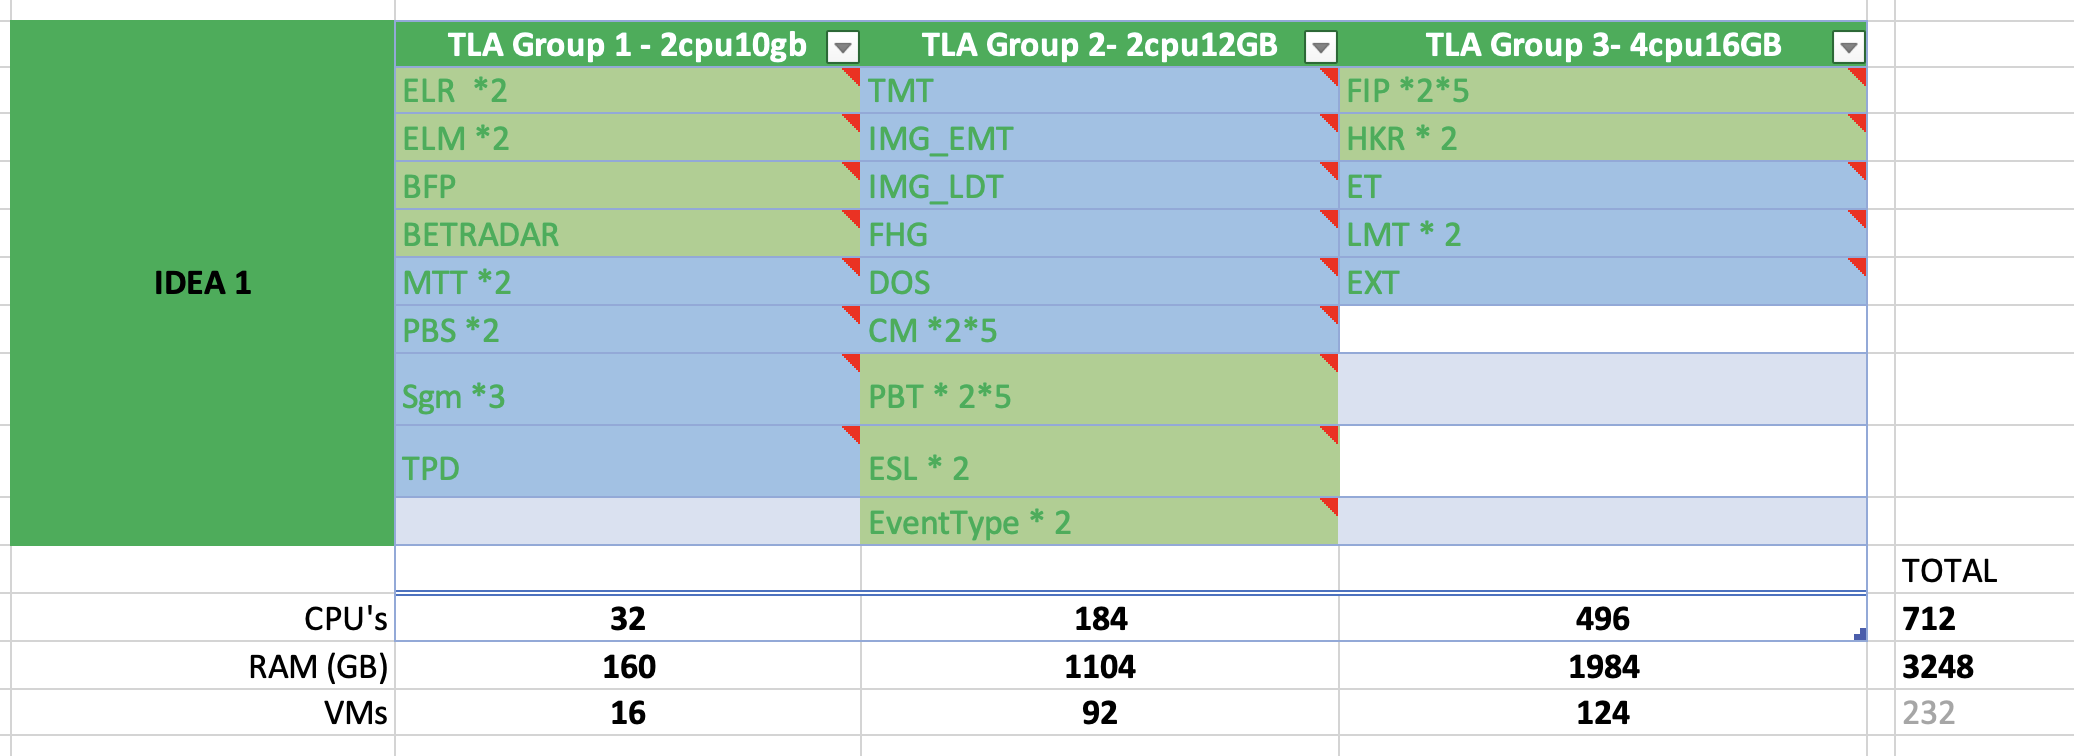
\includegraphics[scale=0.4]{media/content/analise/proposal-1.png}}
  \caption{Distribuição de topologias pelos \textit{clusters} - Alternativa 1}
  \label{proposal-1}
\end{figure}

\subsection{Alternativa 2}

A segunda alternativa, representada na Figura \ref{proposal-2}, diminui a memória RAM utilizada no
primeiro \gls{cluster}, além de reformular a organização das topologias pelos restantes. 

O número de \ac{VM} hospedadas no mesmo \gls{cluster} não deve ser demasiado elevado de forma a
evitar uma carga demasiado elevada no processo de implantação, isto porque, devido à forma como 
funciona o \textit{Apache Storm} a alteração numa topologia implica o processo de implantação de
todo o \gls{cluster} e, logicamente, quanto maior a quantidade de \ac{VM} que devem ser criadas
durante o processo, mais demorado se tornará.

\begin{figure}[H]
  \centerline{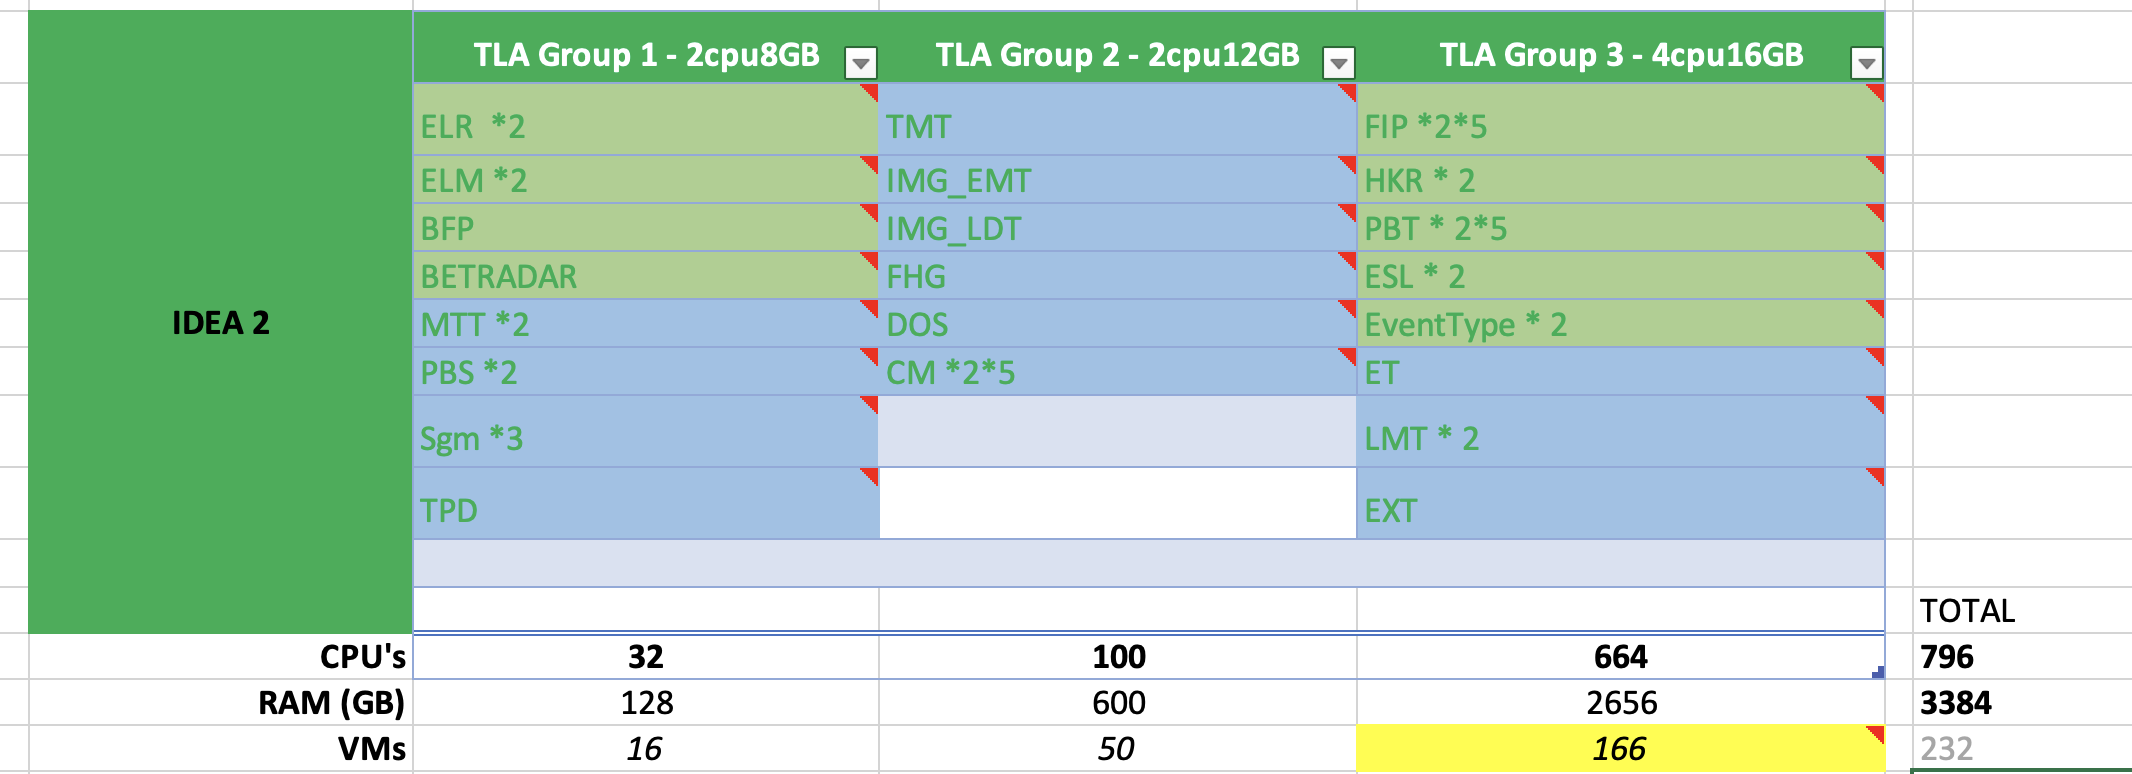
\includegraphics[scale=0.4]{media/content/analise/proposal-2.png}}
  \caption{Distribuição de topologias pelos \textit{clusters} - Alternativa 2}
  \label{proposal-2}
\end{figure}

Esta abordagem acaba por ser inferior às restantes por duas questões - o tamanho, em termos de número 
de \ac{VM}, do terceiro \gls{cluster} e a quantidade total de recursos superior à proposta
analisada anteriormente.

\subsection{Alternativa 3}

A terceira, e última, alternativa está representada na Figura \ref{proposal-3}.

\begin{figure}[H]
  \centerline{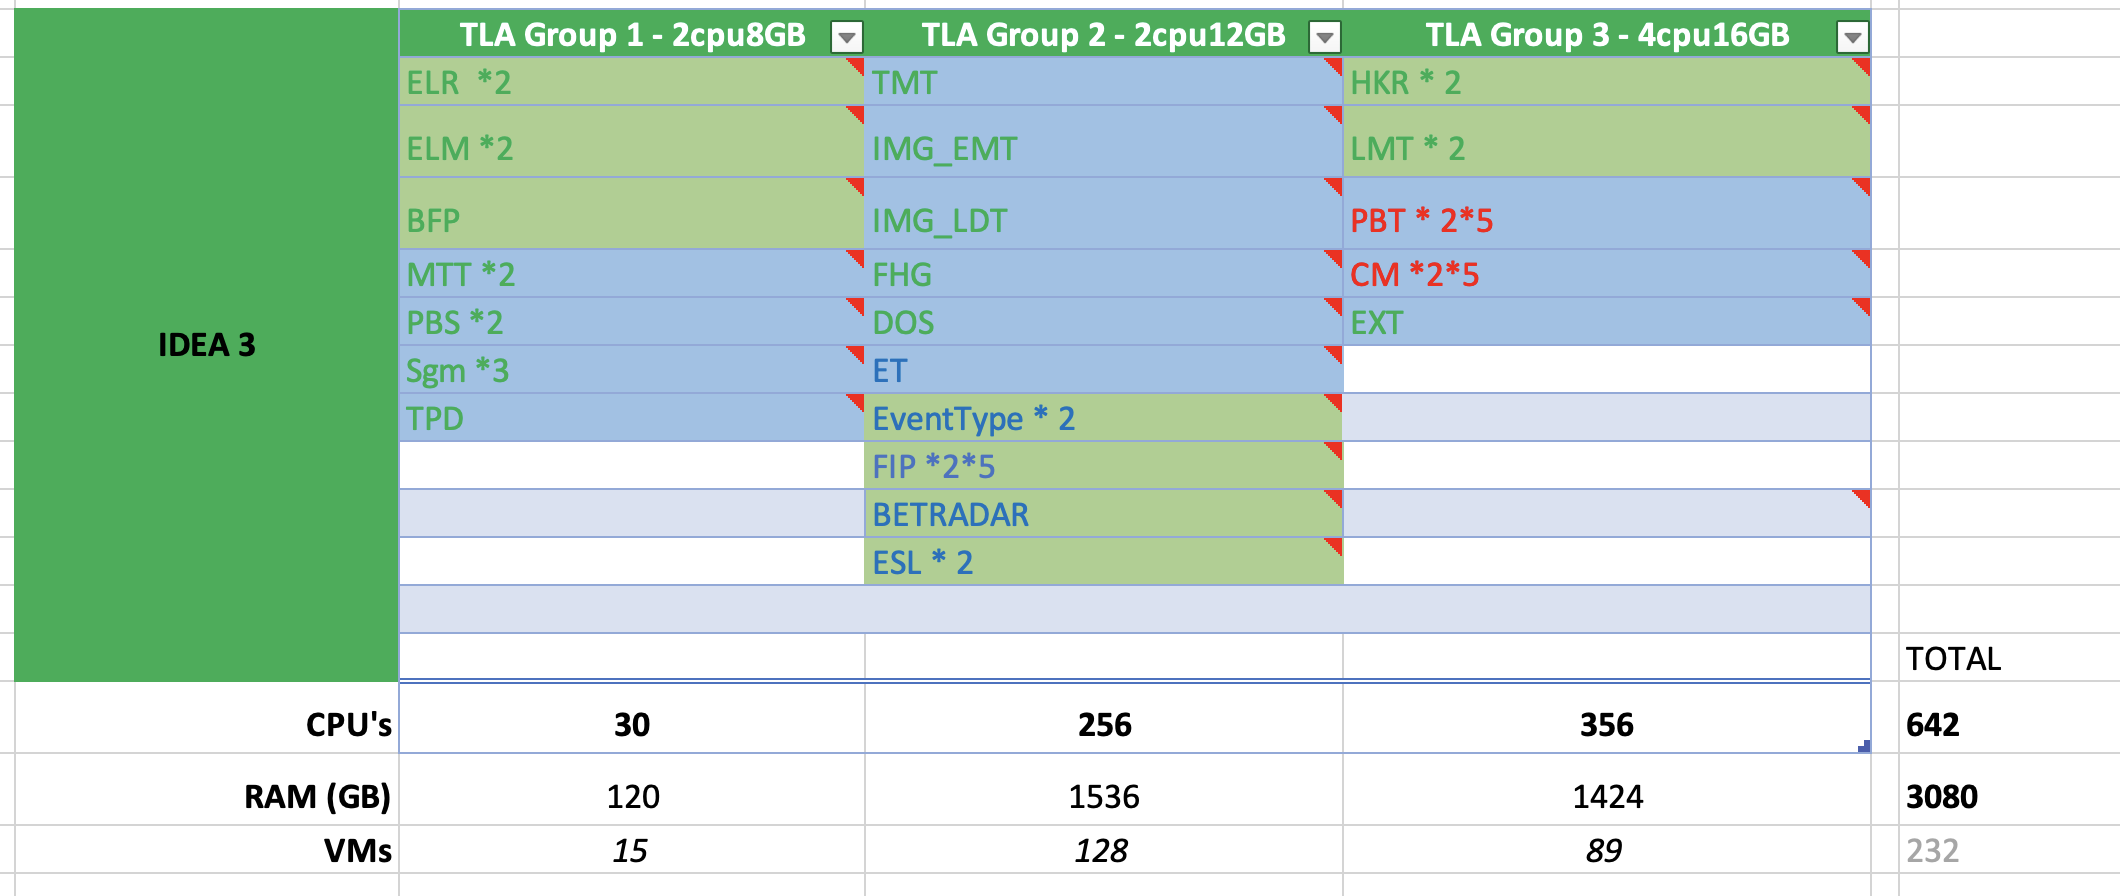
\includegraphics[scale=0.4]{media/content/analise/proposal-3.png}}
  \caption{Distribuição de topologias pelos \textit{clusters} - Alternativa 3}
  \label{proposal-3}
\end{figure}

Esta alternativa acaba por ser a mais vantajosa em quase todos os aspetos, mas acabou por ser 
descartada devido após análise por parte das equipas que desenvolvem as topologias. Isto porque uma 
das topologias é uma exceção às restantes no sentido em que todas as restantes, como mencionado 
anteriormente, na secção de \nameref{sec:3-restricao-design}, a paralelização só é permitida ser 
efetuada por máquina, ou seja, a mesma máquina não pode correr mais que um processo da topologia, 
paralelamente. Devido à necessidade acima do normal de paralelização por parte desta topologia em 
específico acabou por ser aberta a exceção e neste caso cada máquina corre dois processos em 
paralelo. Desta forma, a análise efetuada anteriormente não pode ser interpretada da mesma forma 
para esta topologia, o que invalida esta alternativa.

\subsection{Comparação entre alternativas}

Após uma análise cuidada de todas estas alternativas acabou por ser escolhida a primeira alternativa
com a alteração da memória RAM do primeiro \gls{cluster} chegando à opção ilustrada na Figura
\ref{proposal-final}.

\begin{figure}[H]
  \centerline{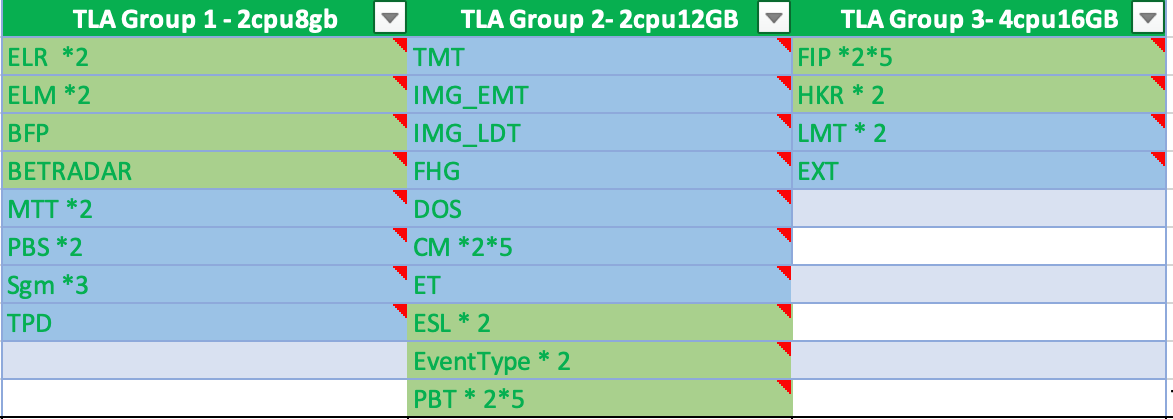
\includegraphics[scale=0.6]{media/content/analise/proposal-final.png}}
  \caption{Distribuição de topologias pelos \textit{clusters} - Alternativa Final}
  \label{proposal-final}
\end{figure}

Podemos observar na Figura \ref{comparison-proposal} a comparação entre todas as propostas
analisadas em termos de uso total de recursos em todos os ambientes, bem como a percentagem de 
redução de recursos em cada um dos parâmetros analisados (CPU e RAM).

\begin{figure}[H]
  \centerline{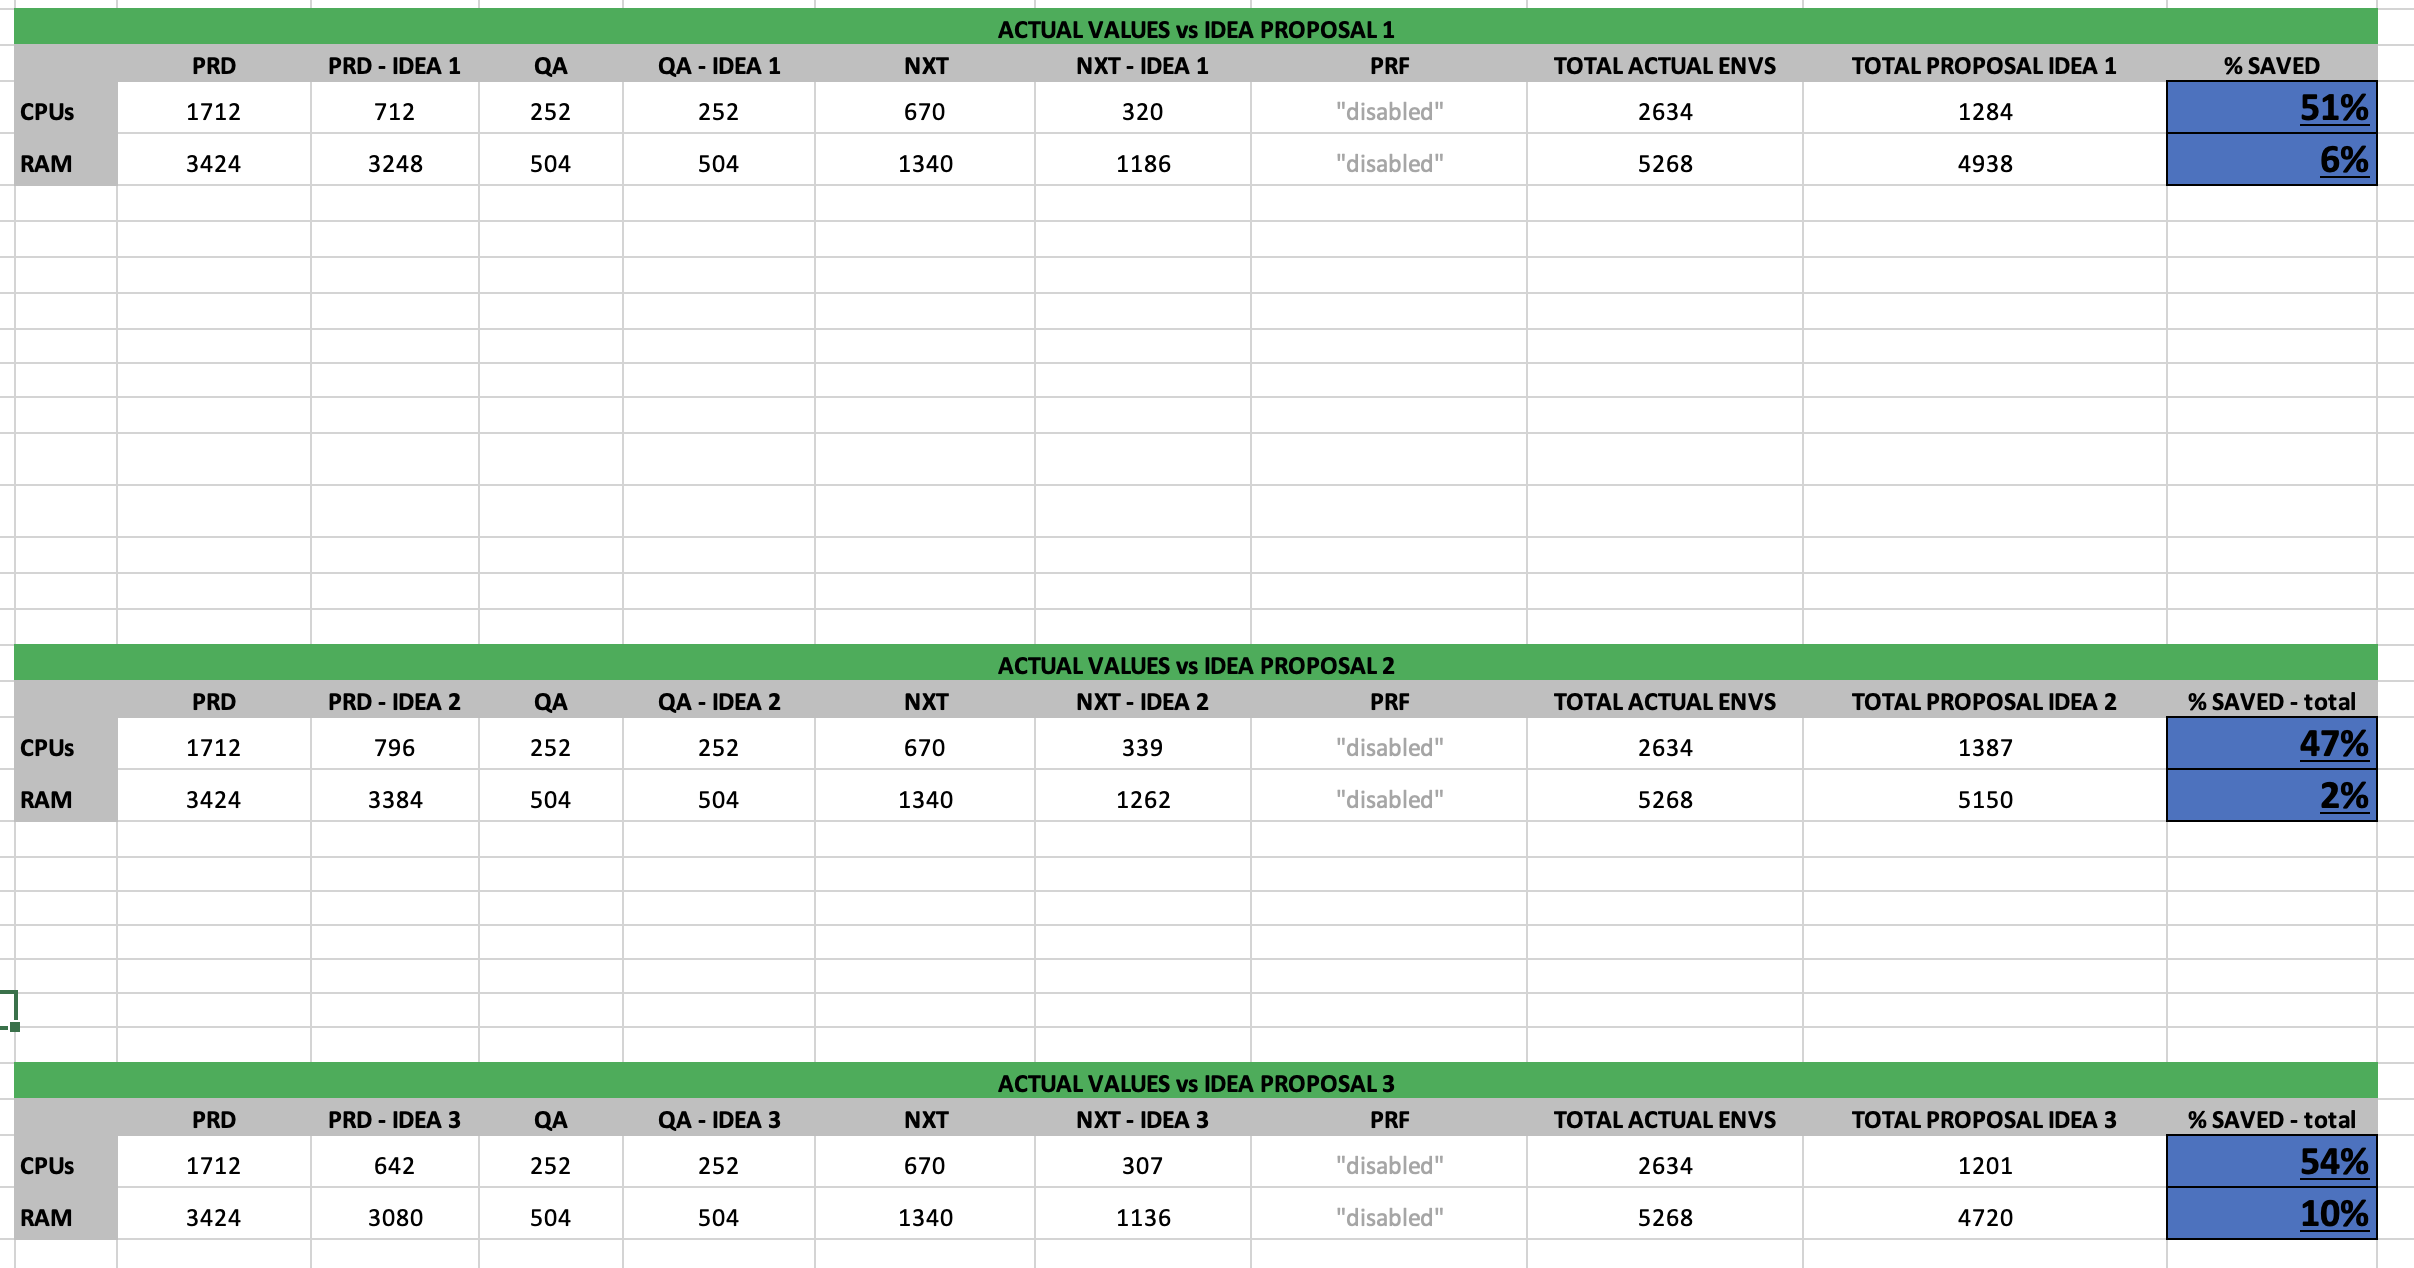
\includegraphics[scale=0.4]{media/content/analise/proposal-comparison.png}}
  \caption{Comparação de propostas de atualização}
  \label{comparison-proposal}
\end{figure}

\section{Processo de implantação}

Após decidir qual a abordagem a ser seguida é necessário definir o processo de implantação a ser
seguido. Este processo deve ser claro e conciso de forma a garantir que todas as equipas envolvidas
compreendam o processo que vai ser implementado e, desta forma, maximizar a probabilidade de
sucesso da intervenção. 

Este processo foi dividido em três passos que vão ser descritos e analisados de seguida. Por uma
questão de simplicidade no trabalho de análise, todos os quadros apresentados de seguida têm por 
base apenas os valores de recursos dos ambientes de produção, ou seja, para obter os valores reais
de redução de recursos deve ser necessário ainda ter em conta os recursos dos restantes ambientes
e multiplicar todos os resultados por dois já que todas as alterações devem ser replicadas em 
ambos os \glspl{dc}. Esta simplificação foi feita já que todas estas variáveis adicionais podem 
ser desprezadas dadas as semelhanças entre ambientes e a dimensão total da infraestrutura em
análise.

Como analisado anteriormente, a Figura \ref{strat-current} representa o estado atual dos 
\glspl{cluster}. Este é o ponto de partida para esta intervenção. 

No primeiro passo, representado na Figura \ref{strat-1}, é efetuada uma redução de recursos 
de ambos os \glspl{cluster}. Esta redução parte do princípio de que, sendo possível aplicar a 
solução final apresentada anteriormente, então, por definição, as topologias devem ser capazes de
operar sem problemas usando estes novos \glspl{flavour}. Esta intervenção só por si, representa
46\% de redução no uso total de \ac{CPU} (no ambiente de produção).

\begin{figure}[H]
  \centerline{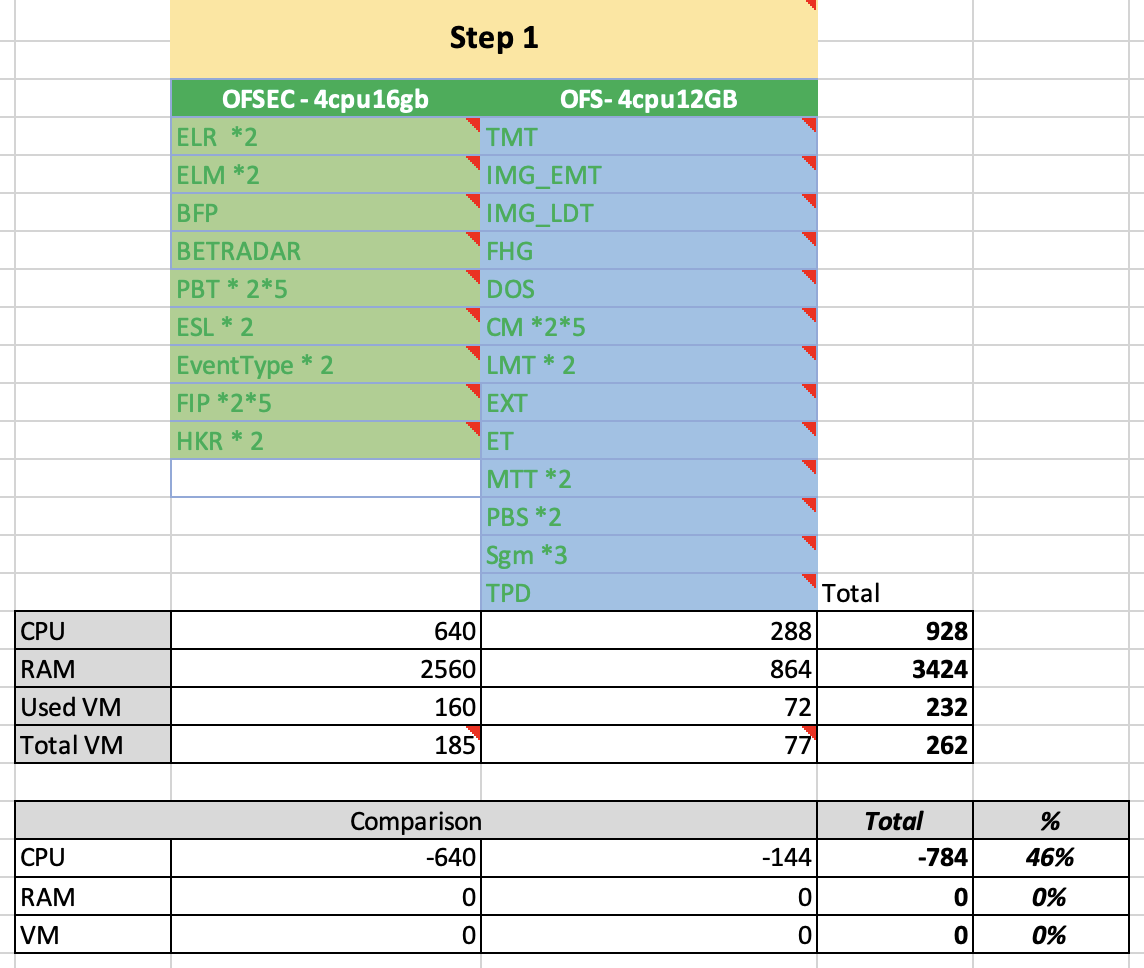
\includegraphics[scale=0.5]{media/content/analise/strat-1.png}}
  \caption{Processo de implantação - Passo 1}
  \label{strat-1}
\end{figure}

O segundo passo foi dividido em duas etapas - a criação do novo \gls{cluster}, representado na 
Figura \ref{strat-2} e a migração das topologias entre \glspl{cluster} (Figura \ref{strat-2_1}).

\begin{figure}[H]
  \centerline{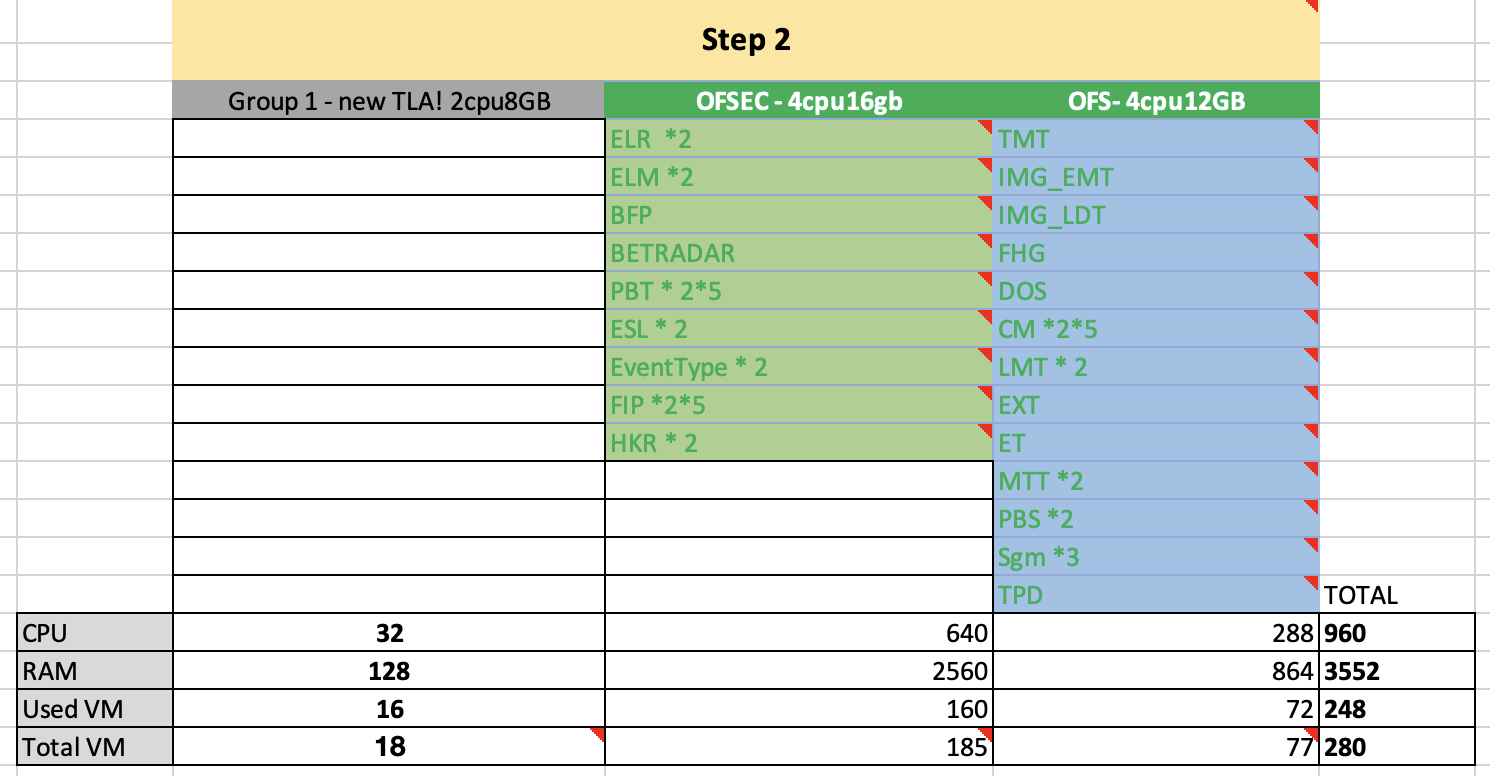
\includegraphics[scale=0.5]{media/content/analise/strat-2.png}}
  \caption{Processo de implantação - Passo 2}
  \label{strat-2}
\end{figure}

A segunda etapa deste passo é a etapa mais crítica de todo o processo, isto porque, nesta fase, é
crucial ter a total compreensão dos processos de replicação e \gls{failover} de cada topologia de
forma a minimizar o tempo de indisponibilidade de cada serviço.

\begin{figure}[H]
  \centerline{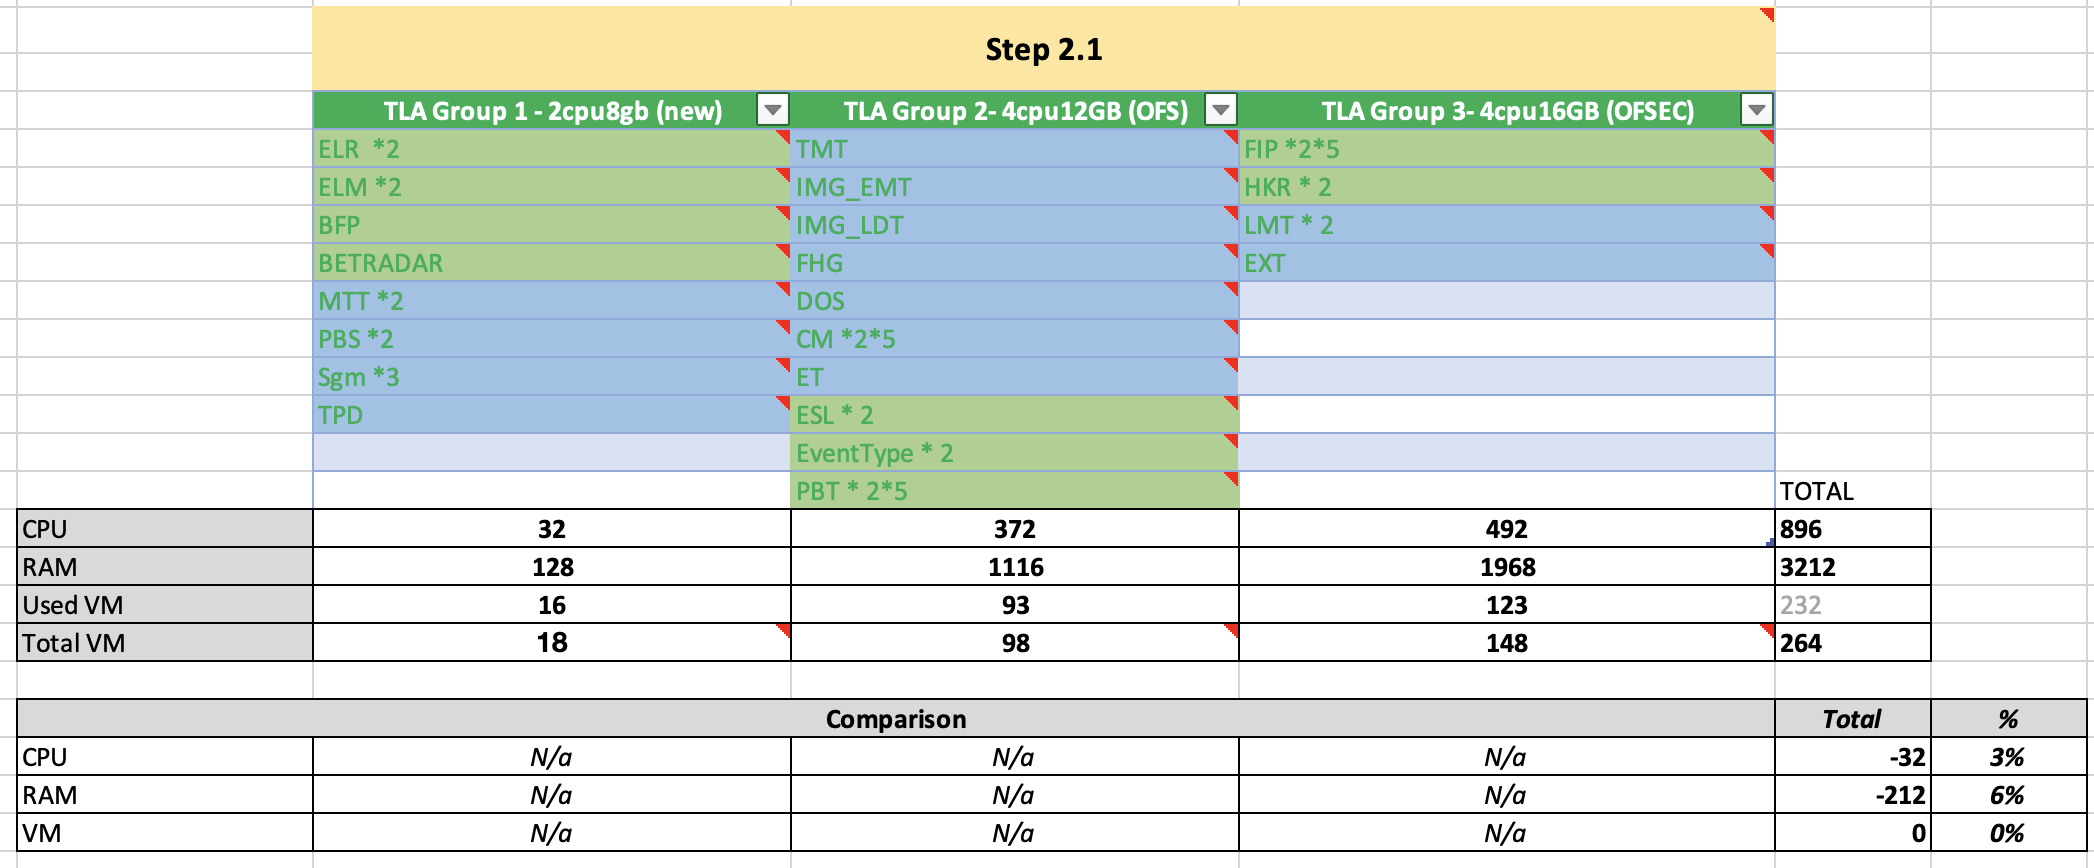
\includegraphics[scale=0.4]{media/content/analise/strat-2_1.png}}
  \caption{Processo de implantação - Passo 2.1}
  \label{strat-2_1}
\end{figure}

O terceiro, e último, passo, representando na Figura \ref{strat-3}, representa uma nova redução 
do \gls{flavour} de um dos \glspl{cluster}. Este passo é em todo semelhante ao primeiro, mas é
apenas necessário efetuar esta redução no segundo \gls{cluster}.

\begin{figure}[H]
  \centerline{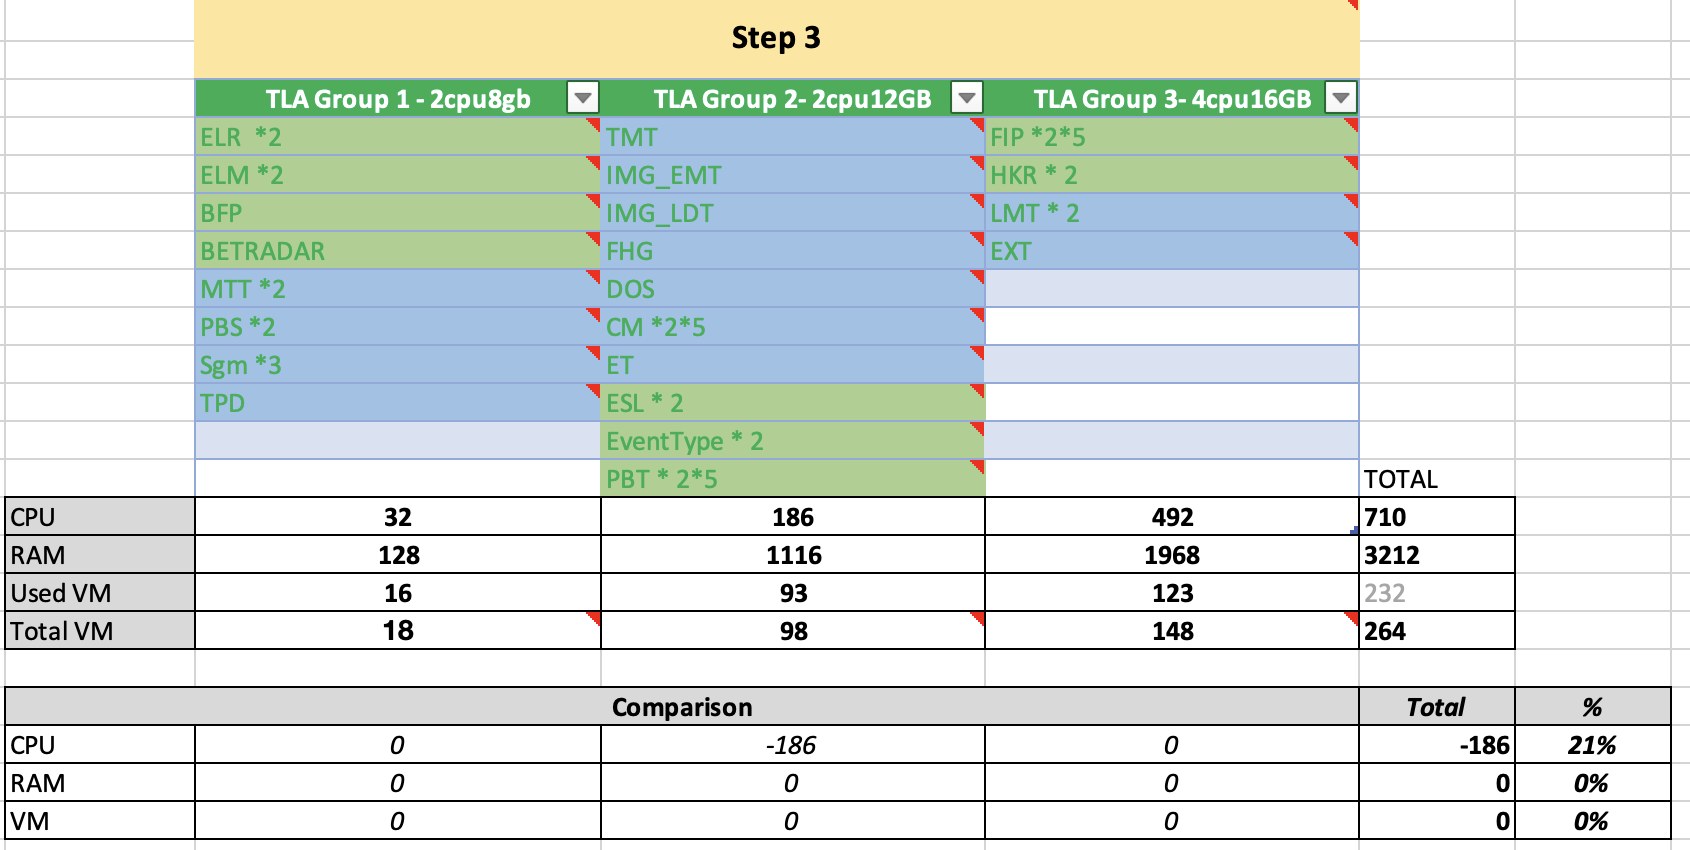
\includegraphics[scale=0.5]{media/content/analise/strat-3.png}}
  \caption{Processo de implantação - Passo 3}
  \label{strat-3}
\end{figure}

De forma a ser mais simples acompanhar as alterações efetuadas em cada passo, uma visualização
com a comparação simplificada está disponível no Anexo \ref{appedix-b}.

Após todo este processo a estrutura em que estão hospedadas as topologias encontra-se na forma
otimizada proposta anteriormente. Este processo sofre pequenas alterações entre ambientes já que 
os \glspl{flavour} não são iguais entre estes. Além disso, durante este processo tiveram que ser 
analisadas outras questões igualmente relevantes para garantir que esta migração era possível como 
é o caso da capacidade de comunicação do \textit{Zookeeper}.

O \textit{Zookeeper} é utilizado por todos estes \glspl{cluster} para garantir a resiliência das 
topologias e, por consequência, poderia não ter a capacidade de comunicar com um \gls{cluster}
adicional. Após analisar esta questão com as equipas responsáveis pela infraestrutura foi 
determinado que esta questão representava um problema crítico para o desempenho do 
\textit{Zookeeper}, logo, a proposta foi aprovada.

